%% Begin slides template file
\documentclass[11pt,t,usepdftitle=false,aspectratio=169]{beamer}
%% ------------------------------------------------------------------
%% - aspectratio=43: Set paper aspect ratio to 4:3.
%% - aspectratio=169: Set paper aspect ratio to 16:9.
%% ------------------------------------------------------------------

\usepackage{tikz}
\usetikzlibrary{snakes}
\usepackage{pgfgantt}
\usepackage{multicol}

\usepackage[
backend=biber,
style=alphabetic,
citestyle=alphabetic
]{biblatex}

\addbibresource{literature.bib}

\usetheme[nototalframenumber,foot,logo]{uibk}
%% ------------------------------------------------------------------
%% - foot: Add a footer line for conference name and date.
%% - logo: Add the university logo in the footer (only if 'foot' set).
%% - bigfoot/sasquatch: Larger font size in footer.
%% - nototalslidenumber: Hide the total number of slides (only if 'foot' set)
%% - license: Add CC-BY license symbol to title slide (e.g., for conference uploads)
%%   (TODO: At the moment no other licenses are supported.)
%% - licenseall: Add CC-BY license symbol to all subsequent slides slides
%% - url: use \url{} rather than \href{} on the title page
%% ------------------------------------------------------------------

%% ------------------------------------------------------------------
%% The official corporate colors of the university are predefined and
%% can be used for e.g., highlighting something. Simply use
%% \color{uibkorange} or \begin{color}{uibkorange} ... \end{color}
%% Defined colors are:
%% - uibkblue, uibkbluel, uibkorange, uibkorangel, uibkgray, uibkgraym, uibkgrayl
%% The frametitle color can be easily adjusted e.g., to black with
%% \setbeamercolor{titlelike}{fg=black}
%% ------------------------------------------------------------------

%\setbeamercolor{verbcolor}{fg=uibkorange}
%% ------------------------------------------------------------------
%% Setting a highlight color for verbatim output such as from
%% the commands \pkg, \email, \file, \dataset 
%% ------------------------------------------------------------------


%% information for the title page ('short title' is the pdf-title that is shown in viewer's titlebar)
\title[Analysis]{Longitudinal Analysis of SSH Honeypot Logs}
\subtitle{Security and Privacy Lab, Department of Computer Science}
% \text{Supervisor: Maximilian Hils}
% \URL{www.uibk.ac.at/statistics}

\author[Dominic Rudigier]{Dominic Rudigier, 11832156  |  Supervisor: Maximilian Hils}
%('short author' is the pdf-metadata Author)
%% If multiple authors are required and the font size is too large you
%% can overrule the font size of author and url by calling:
%\setbeamerfont{author}{size*={10pt}{10pt},series=\mdseries}
%\setbeamerfont{url}{size*={10pt}{10pt},series=\mdseries}
%\URL{}
%\subtitle{}

\footertext{Longitudinal Analysis of SSH Honeypot Logs}
\date{2021-05-11}

\headerimage{3}
%% ------------------------------------------------------------------
%% The theme offers four different header images based on the
%% corporate design of the university of innsbruck. Currently
%% 1, 2, 3 and 4 is allowed as input to \headerimage{...}. Default
%% or fallback is '1'.
%% ------------------------------------------------------------------

\begin{document}

%% ALTERNATIVE TITLEPAGE
%% The next block is how you add a titlepage with the 'nosectiontitlepage' option, which switches off
%% the default behavior of creating a titlepage every time a \section{} is defined.
%% Then you can use \section{} as it's originally intended, including a table of contents.
% \usebackgroundtemplate{\includegraphics[width=\paperwidth,height=\paperheight]{titlebackground.pdf}}
% \begin{frame}[plain]
%     \titlepage
% \end{frame}
% \addtocounter{framenumber}{-1}
% \usebackgroundtemplate{}}

%% Table of Contents, if wanted:
%% this requires the 'nosectiontitlepage' option and setting \section{}'s as you want them to appear here.
%% Subsections and subordinates are suppressed in the .sty at the moment, search
%% for \setbeamertemplate{subsection} and replace the empty {} with whatever you want.
%% Although it's probably too much for a presentation, maybe for a lecture.
% \begin{frame}
%     \vspace*{1cm plus 1fil}
%     \tableofcontents
%     \vspace*{0cm plus 1fil}
% \end{frame}


%% this sets the first PDF bookmark and triggers generation of the title page
\section{Longitudinal Analysis of SSH Honeypot Logs}

%% this just generates PDF bookmarks
\subsection{Motivation}
\begin{frame}
	\frametitle{Motivation}	
	\begin{center}
	
\includegraphics[width=20mm]{_images/honeypot.png}
	\end{center}
	\begin{center}
	
\includegraphics[width=20mm]{_images/head_question.png}
	\end{center}
\end{frame}
\begin{frame}
\frametitle{Motivation}	
\begin{center}
	
\includegraphics[width=90mm]{_images/Visualization_Honeypot_Bear.png}
\end{center}
\end{frame}
%% first slide
\begin{frame}
	\frametitle{Motivation}
	
	\textbf{Honeypot:}
	\begin{itemize}
		\item Mimics easy target and attracts attackers
		\item Generates logs about connection data (commands, files uploaded)
		\item Gained information can be used to improve systems		
	\end{itemize}
	\pause
	 \begin{exampleblock}{Example}
	 	\begin{enumerate}
	 		\item Hardcoded credentials in software
	 		\item Attacker found out somehow
	 		\item Analyzing honeypot logs shows that hacker knows
	 		\item Operator can react to vulnerability
	 	\end{enumerate}
	\end{exampleblock}
\end{frame}
\begin{frame}[fragile]
	\frametitle{Motivation}	
	\begin{center}
		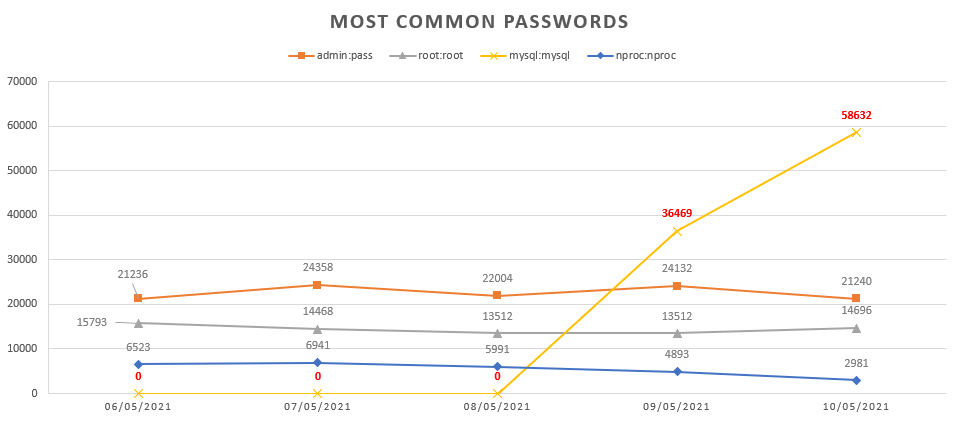
\includegraphics[width=120mm]{_images/Visualization_Common_Passwords_Anomalie.png}
	\end{center}
\end{frame}

\begin{frame}
	\frametitle{Motivation}	
	\begin{center}
		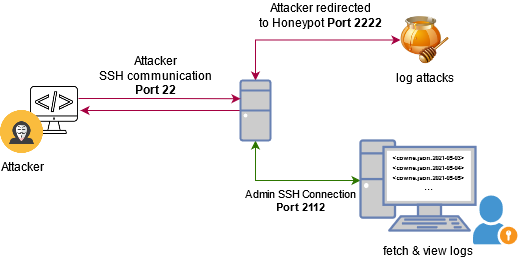
\includegraphics[width=110mm]{_images/SSH_Overview.png}
	\end{center}
\end{frame}
	%%\textbf{Problem:} Too much information gathered, hard to handle.

\subsection{Status quo}
\begin{frame}
	\frametitle{Status quo}	
	\textbf{Cowrie:}
	\begin{itemize}
		\item SSH and Telnet honeypot
		\item Different log formats for connection data (JSON, UML, MongoDB,..)
	\end{itemize}
	
	\begin{alertblock}{Problem}
		\begin{itemize}
			\item Malware has become more intelligent 
			\item e.g. Aisuru detects Cowrie honeypots
			\begin{itemize}
				\item existence of "@LocalHost:]"
				\item existence of a service, started on Jun 22nd, or Jun 23rd
				\item user exists on the device named "richard"
			\end{itemize}
			\item Improve honeypot configurations
		\end{itemize}
	\end{alertblock}	
\end{frame}

\begin{frame}
	\frametitle{Status quo}
	
	\textbf{Already existing:}
	\begin{itemize}
		\item SSH Session Playback (single connection)
		\item Data analyzation platforms (aggregated statistics)
	\end{itemize}
	
	\begin{alertblock}{Problem}
		\begin{itemize}
			\item Providers
			\begin{itemize}
				\item Multiple thousands of honeypots 
				\item Each honeypot logs thousands of attacks per hour
				\item Too much information gathered, hard to handle.
			\end{itemize}
		\end{itemize}
	\end{alertblock}	
\end{frame}
%%%%
\subsection{Thesis contribution}
\begin{frame}
\frametitle{Thesis contribution}
\begin{center}
	
\includegraphics[width=140mm]{_images/Motivation_Overview.png}
\end{center}
\end{frame}
%%%%
\begin{frame}
	\frametitle{Thesis contribution}	
	\textbf{Longitudinal analysis:}
	\begin{itemize}
		\item Research design that involves repeated observations of the same variables.		
		\item Research attacker behaviour over time.
	\end{itemize}	
	\begin{block}{Batch-processing of log files}
		\begin{enumerate}
			\item Cowrie generates log files \textbf{<cowrie.json.2021-05-01, 100 to 200 MB>}
			\begin{itemize}
				\item per honeypot (instance)
				\item per day (multiple)
				\item 1k honeypots / 30 days = 3-6 TB log data per month
			\end{itemize} 
			\item Batch-process using MapReduce model with Python
			\item Visualize (Python or Flask + ReactJS)	
		\end{enumerate}
	\end{block}
\end{frame}
%%

%\begin{frame}[fragile]
%	\frametitle{Batch-processing of log files}
%
%\textbf{cowrie.json.2021-05-01:} Log files for each honeypot each day
%
%\bigskip
%\begin{tabular}{l}
%	\hline
%	Generated logs  \\
%	\hline
%	\verb|{"eventid":"cowrie.session.connect","src_ip":"5.253.24.65" ..|      \\
%	\verb|{"eventid":"cowrie.client.version","version":"b'SSH-2.0-li ..|   \\
%	\verb|{"eventid":"cowrie.client.kex","hassh":"51cba57125523ce4b9 ..|      \\
%	\verb|{"eventid":"cowrie.login.failed","username":"minecraft","p ..|   \\
%	\verb|{"eventid":"cowrie.session.closed","duration":1.7365803718 ..|     \\
%	\verb|{"eventid":"cowrie.command.input","input":"cat /proc/cpuin ..|    \\
%	\hline
%\end{tabular}
%
%
%\end{frame}
%
%%%%%  
%\subsection{Batch-processing of log files}
%\begin{frame}[fragile]
%	\frametitle{Batch-processing of log files}		
%	\textbf{MapReduce:} Programming model for performant data analysis
%	
%	\bigskip	 
%	
%	\begin{tabular}{ll}
%		\hline
%		Procedure & Functionality \\
%		\hline
%		\verb|\split_func{...}|     & split into JSON objects \\
%		\verb|\map_func{...}|     & map, filter and sort objects \\
%		\verb|\reduce_func{...}|   & aggregate event data to summary \\
%		\hline
%	\end{tabular}
%\end{frame}
%
%\begin{frame}[fragile]
%	\frametitle{Batch-processing of log files}	
%	\begin{tabular}{ll}
%		\hline
%		Method & Output \\
%		\hline
%		Input & \verb|{"eventid":"cowrie.session.connect", "user":"..}| \\
%		Map & \verb|[(2021-05-01:root:root, 1), (..), ...]|	  \\
%		Reduce & \verb|{ |  \\
%			& \verb|  honeypot: "honeypotA",|  \\
%			& \verb|  date: "2021-04-25", |   \\
%			& \verb|  passwords: [ {user: "root", password: "root", |  \\
%				& \verb|  count: 14476}, ... ] /* top N attempts today */|  \\
%			& \verb|}|  \\ 
%		\hline
%	\end{tabular}
%\end{frame}

\begin{frame}[fragile] 
	\frametitle{Batch-processing of log files}	
	% \textbf{MapReduce:} Programming model for performant data analysis
	\begin{columns}
		\begin{column}{0.3\textwidth}
		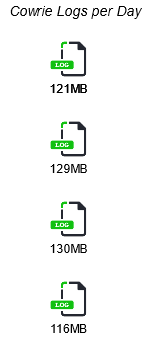
\includegraphics[width=18mm\textwidth]{_images/MapReduce-Visualization-01.png}
		\end{column}	
		\begin{column}{0.7\textwidth}
			\begin{tabular}{l}
			\hline
			cowrie.json.2021-05-01  \\
			\hline
			\verb|{"eventid":"cowrie.session.connect","src_ip..|      \\
			\verb|{"eventid":"cowrie.client.version","version..|   \\
			\verb|{"eventid":"cowrie.login.failed","usernamem..|   \\
			\verb|{"eventid":"cowrie.session.closed","duration..|     \\
			\verb|{"eventid":"cowrie.command.input","input..|    \\
				\hline
			\end{tabular}
		\end{column}
	\end{columns}
\end{frame}

\begin{frame}[fragile]
	\frametitle{Batch-processing of log files}	
	\begin{center}
		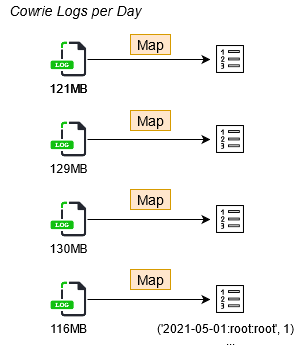
\includegraphics[width=45mm]{_images/MapReduce-Visualization-02.png}
	\end{center}
\end{frame}

\begin{frame}[fragile]
	\frametitle{Batch-processing of log files}	
	\begin{center}
		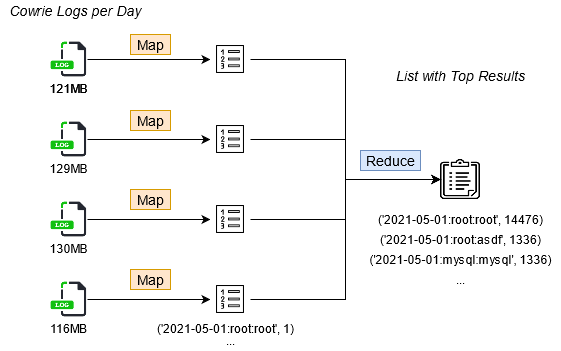
\includegraphics[width=90mm]{_images/MapReduce-Visualization-03.png}
	\end{center}
\end{frame}

\begin{frame}[fragile]
	\frametitle{Batch-processing of log files}	
	\begin{center}
		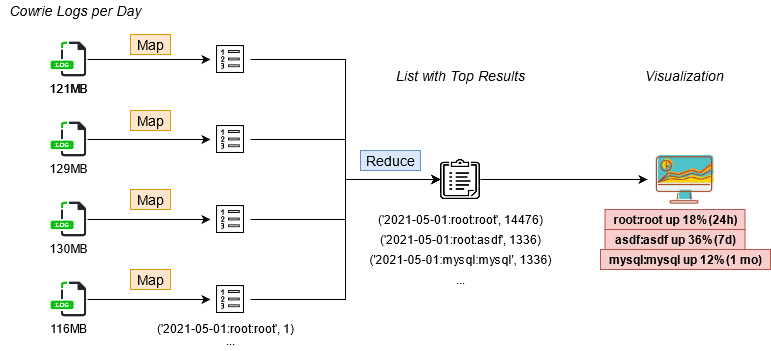
\includegraphics[width=120mm]{_images/MapReduce-Visualization-04.png}
	\end{center}
\end{frame}


\subsection{Goal}
\begin{frame}
	\frametitle{Goal}
	\textbf{Extract information:}
	\begin{enumerate}
		\item Detect changes in attacker behavior over time		
		\begin{exampleblock}{Changes over time might indicate new vulnerabilities}
			\begin{itemize}
				\item User:Password combination changes
				\item Commands executed before disconnect 
				\item Command quantity changes
				\item All log anomalies not previously shown up
			\end{itemize}
		\end{exampleblock}
		\item Visualize 
		\item Find ways to improve honeypot configurations 
	\end{enumerate}
\end{frame}
%%%%  
\subsection{Timeline}
\begin{frame}
	\frametitle{Timeline}
	\begin{ganttchart}[
		hgrid,
		vgrid={*{6}{draw=none},{dotted}},
		x unit=0.05cm,
		y unit title=0.5cm,
		y unit chart=0.5cm,
		title label font=\fontsize{4}{5}\selectfont,
		bar label font=\tiny,
		bar/.append style={fill=green!60},
		bar incomplete/.append style={fill=green!7},
		progress label text={""},
		group label font=\tiny\bfseries,
		milestone label font=\tiny\itshape,
		time slot format=isodate
		]{2021-03-01}{2021-08-31}
		\gantttitlecalendar{year, month=name} \\			
		\ganttbar[progress=100]{Research ssh honeypots}{2021-03-1}{2021-03-7} \\
		\ganttbar[progress=100]{Cowrie setup, test Splunk}{2021-03-8}{2021-03-15} \\
		\ganttbar[progress=100]{Tried mongoDB for logs}{2021-03-16}{2021-04-1} \\
		\ganttbar[progress=100]{Research batch-process / MapReduce}{2021-04-2}{2021-04-15} \\
		\ganttbar[progress=85]{Implement/Visualize MapReduce}{2021-04-16}{2021-05-15} \\
		\ganttbar[progress=0]{Extend to multiple anomalies / Visualize}{2021-05-16}{2021-06-15} \\
		\ganttbar[progress=0]{Handle bugs / improvements}{2021-06-16}{2021-06-30} \\
		\ganttbar[progress=0]{Generate hints to improve honeypots}{2021-07-01}{2021-07-15} \\
		\ganttbar[progress=0]{Write thesis}{2021-07-16}{2021-08-30} 
		\ganttlink{elem0}{elem1}
		\ganttlink{elem1}{elem2}
		\ganttlink{elem2}{elem3}
		\ganttlink{elem3}{elem4}
		\ganttlink{elem4}{elem5}
		\ganttlink{elem6}{elem7}
		\ganttlink{elem7}{elem8}
	\end{ganttchart}
\end{frame}

\subsection{References}
% bibliography
\begin{frame}[allowframebreaks]
	\frametitle{References}
	%\bibliographystyle{amsalpha}
	\nocite{*}
	\printbibliography
\end{frame}

%%
%% to show a last slide similar to the title slide: information for the last page
\title{Thank you for your attention!}
\subtitle{}
\section{Thanks}


%% appendix of 'extra' slides
\appendix

\begin{frame}
\frametitle{Appendix 1}
    \url{https://www.sicherheitstacho.eu/start/main} \\
    \url{https://www.avira.com/en/blog/new-mirai-variant-aisuru-detects-cowrie-opensource-honeypots}
\end{frame}

%\begin{frame}
%\frametitle{Appendix 2}
%    This slide does not increase the total number of slides and can hold additional information
%    that you may be asked about after the end of the presentation.
%\end{frame}

\end{document}

